\documentclass{article}                                                   %
\usepackage{fullpage}                                                     %
\usepackage{pgffor}                                                       %
\usepackage{amssymb}                                                      %
\usepackage{Sweave}                                                       %
\usepackage{bm}                                                           %
\usepackage{mathtools}                                                    %
\usepackage{verbatim}                                                     %
\usepackage{appendix}                                                     %
\usepackage[UKenglish]{isodate} % for: \today                             %
\cleanlookdateon                % for: \today                             %
                                                                          %
\def\wl{\par \vspace{\baselineskip}}                                      %
\def\beginmyfig{\begin{figure}[htbp]\begin{center}}                       %
\def\endmyfig{\end{center}\end{figure}}                                   %
                                                                          %
\begin{document}                                                          %
% my title:                                                               %
\begin{center}                                                            %
  \section*{\textbf{Stat536 Midterm - Ozone Data}}                        %
  \subsection*{\textbf{Arthur Lui}}                                       %
  \subsection*{\noindent\today}                                           %
\end{center}                                                              %
\setkeys{Gin}{width=1\textwidth}                                          %
%%%%%%%%%%%%%%%%%%%%%%%%%%%%%%%%%%%%%%%%%%%%%%%%%%%%%%%%%%%%%%%%%%%%%%%%%%%

\section{Introduction}
  Ozone (O$_3$), a gas in the atmosphere, protects humans from the sun's UV
  radiation. However, ozone that is close to the ground can be dangerous to
  humans. Ozone is formed when pollutants react with each other in the presence
  of heat. It is the main component of smog. Enhaling high concentrations of
  O$_3$ triggers chest pain, bronchitis, emphysema, asthma, etc. Scientists have
  monitored O$_3$ levels by 1) direct measurement at measurement stations and 2)
  mathematically simulating the measurements using Community Multi-scale Air
  Quality Model (CMAQ). CMAQ O$_3$ measurements are simulated (on a fine spatial
  scale) based on ground characteristics, temperature, urban density, etc.  So,
  CMAQ data is vast (see \textbf{Figure 1}), but not as accurate as direct
  measurements. However, direct measurements are sparse (see \textbf{Figure 2}).
  The Environmental Protection Agency (EPA), which monitors O$_3$ are,
  therefore, interested in understanding the relationship between CMAQ (which is
  inaccurate) and station measurements. They eventually hope to predict
  ground-level O$_3$ at many locations given CMAQ measurements and observed
  measurements. Using a data set provided by Dr.  Heaton, I will construct such
  a model using a Gaussian Process.

  %Exploratory Plots
  \begin{figure}\begin{center}
    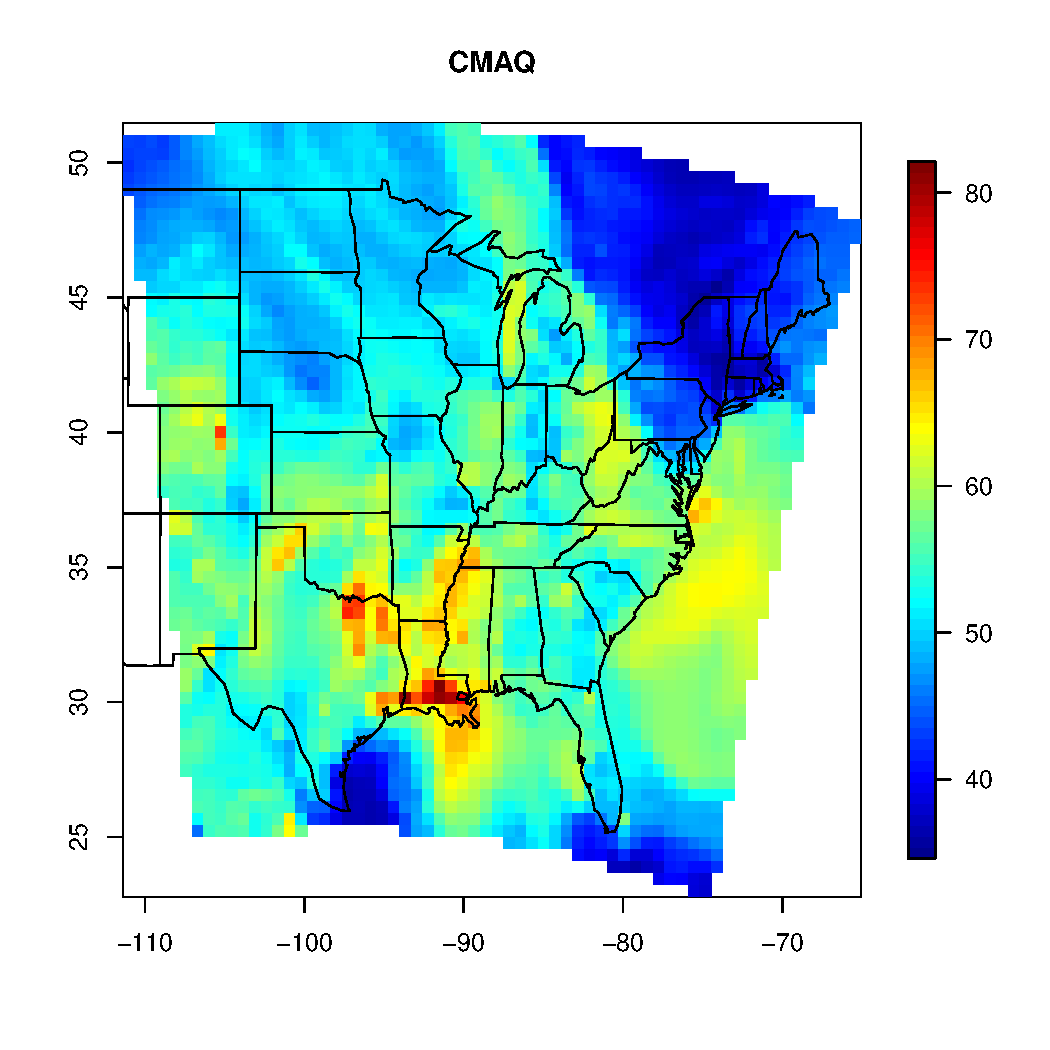
\includegraphics{raw/cmaq.pdf}
    \caption{CMAQ measurements of O$_3$. CMAQ simulates O$_3$ measurements
             easily at many locations. But measurements are inaccurate.}
  \end{center}\end{figure}

  \begin{figure}\begin{center}
    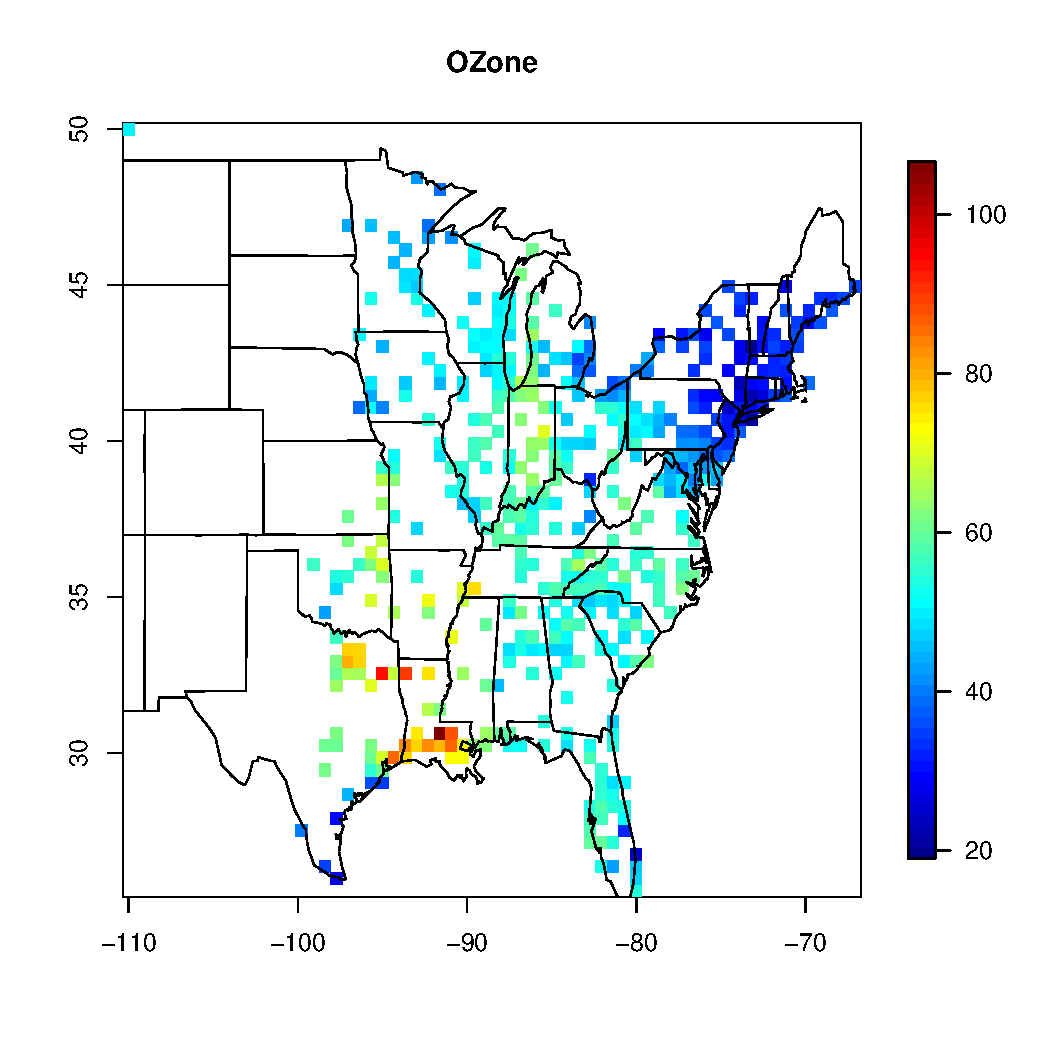
\includegraphics{raw/ozone.pdf}
    \caption{Direct measurements of O$_3$. Direct measurements are sparse.}
  \end{center}\end{figure}


\section{Methods \& Model Used}
  The data received consists of longitude, latitudes, and O$_3$ measurements.
  We are interested in creating a model to predict O$_3$ given CMAQ and grid 
  locations. This is a spatial problem. O$_3$ levels should be highly coorelated 
  to other O$_3$ levels close by, but less correlated to O$_3$ levels far away. 
  But we would like to incorporate CMAQ as a covariate also so that we can
  understand the relationship between directly-measured O$_3$ and CMAQ O$_3$.
  The model we create should also not assume linearity as we are not certain if
  CMAQ and directly-measured O$_3$ are linear. The Gaussian Process Model can
  help us to created such a model. 

  \subsection{Description of The Gaussian Process:}
  A Gaussian Process (GP) is a stochastic process where any finite collection
  observed random variables follow a multivariate normal distribution.
  In other words, for any set of $t_1,\dots,t_N \in T,~\bm{Y} =
  (Y(t_1),\dots,Y(t_N))^T \sim \mathcal{N}(\bm\mu,\bm\Sigma_Y)$.

  % Write out model:
  \subsubsection{Full Gaussian Process Model:}  
    Let N = number of observations and, 
    \[ \bm{Y|W} = \begin{pmatrix} y(x_1) \\ \vdots \\ y(x_N) \end{pmatrix} 
                  \sim \mathcal{N}(\bm W,\tau^2\bm I_N) \]
    \wl
    \[ \bm W =  \begin{pmatrix} w(x_1) \\ \vdots \\ w(x_N) \end{pmatrix}
                \sim \mathcal{N}(\mu\bm 1_N,\sigma^2\bm R) \]
    which marginalizes to:
    \[ \bm Y \sim \mathcal{N}(\mu\bm 1_N,\sigma^2\bm R + \tau^2\bm I_N) \] 
    where,\\
          $\tau^2$ can be interpreted as the error variance; \\
          $\sigma^2$ can be interpreted as the spatial variance; \\
          $ \begin{matrix*}[l]
            \bm R_{ij} & = & \frac{1}{2^{\nu-1}\gamma(\nu)} 
                             (2\phi \sqrt{\nu} |t_i-t_j|)^\nu 
                             K_\nu(2\phi\sqrt{\nu}|t_i-t_j|) \\
                       & = & Matern(|x_i-x_j|,nu=\nu,alpha=\phi) \\
                       & = & Corr(Y(x_i),Y(x_j))
          \end{matrix*} $ \\
          $\phi$: decay parameter. As $\phi$ increases, correlation (at a fixed
          distance) decreases.\\
          $\nu$: smoothness parameter. As $\nu$ increases, smoothness increases.\\
          $K$: effective range. distance where correlation decays to 0.05. \\
          We can estimate the unknown parameters $\mu, \sigma^2, \nu, \phi,
          \tau^2$ (using maximum likelihood or Bayes).
    \wl\noindent
    This is a fascinating result that reduces computation significantly. Making
    use of the properties of the conditional distribution of multivariate normals
    distributions, one can easily can predictions and prediction intervals (see
    Rencher \& Schaalje, Theorem 4.4d, 2008). 
  

  \subsection{Assumptions}
\section{Model Justification}
  \subsection{Why choose a Gaussian Process?}
  The Gaussian Process model incoorporates the spatial distance of the points 
  at which a prediction is made to model nonlinear relationships between a
  response $\bm Y$ and covariates $\bm X$. Since it is the case that we want
  to base our predictions of ozone in this way, where our covariates are some
  linear combination of the nearest CMAQ levels, the Gaussian Process is very
  suitable for this analysis.
  \wl\noindent
  In spatial statistics,y(s), the (functional) response at a grid location,
  is highly nonlinear. We observe $y(s_1),\ldots,y(s_N)$ and the covariates
  $x(s_1),\ldots,x(s_N)$ at N distinct spatial locations $s_1,\ldots,s_N$
  in some spatial region $\mathcal{D}$.
  We can set up the Spatial Statistics Model in this way:
  \[ \bm Y = \begin{pmatrix} y(s_1) \\ \vdots \\ y(s_N) \end{pmatrix} 
             \sim \mathcal{N}(\bm{X\beta},\sigma^2\bm R + \tau^2\bm I_N) \] 
  where,  \begin{itemize}
            \item $\bm Y$ = Station Measured OZone
            \item $\bm X$ = the 10 CMAQ values nearest to our prediction location
            \item $\bm\beta$ = a vector of constants to be estimated
            \item $\bm R_{ij}$ = $\prod_{p=1}^P$ 
                                 Matern(||$\bm{s_{ip}-s_{jp}}$||,$\nu$,$\phi$), 
            \item $\phi,\nu,\sigma^2, and \tau^2$ can be estimated using 
                                                  maximum likelihood.
          \end{itemize}
         

  \subsection{Are Assumptions Justified?}
    %\includegraphics{raw/resids.pdf}
    %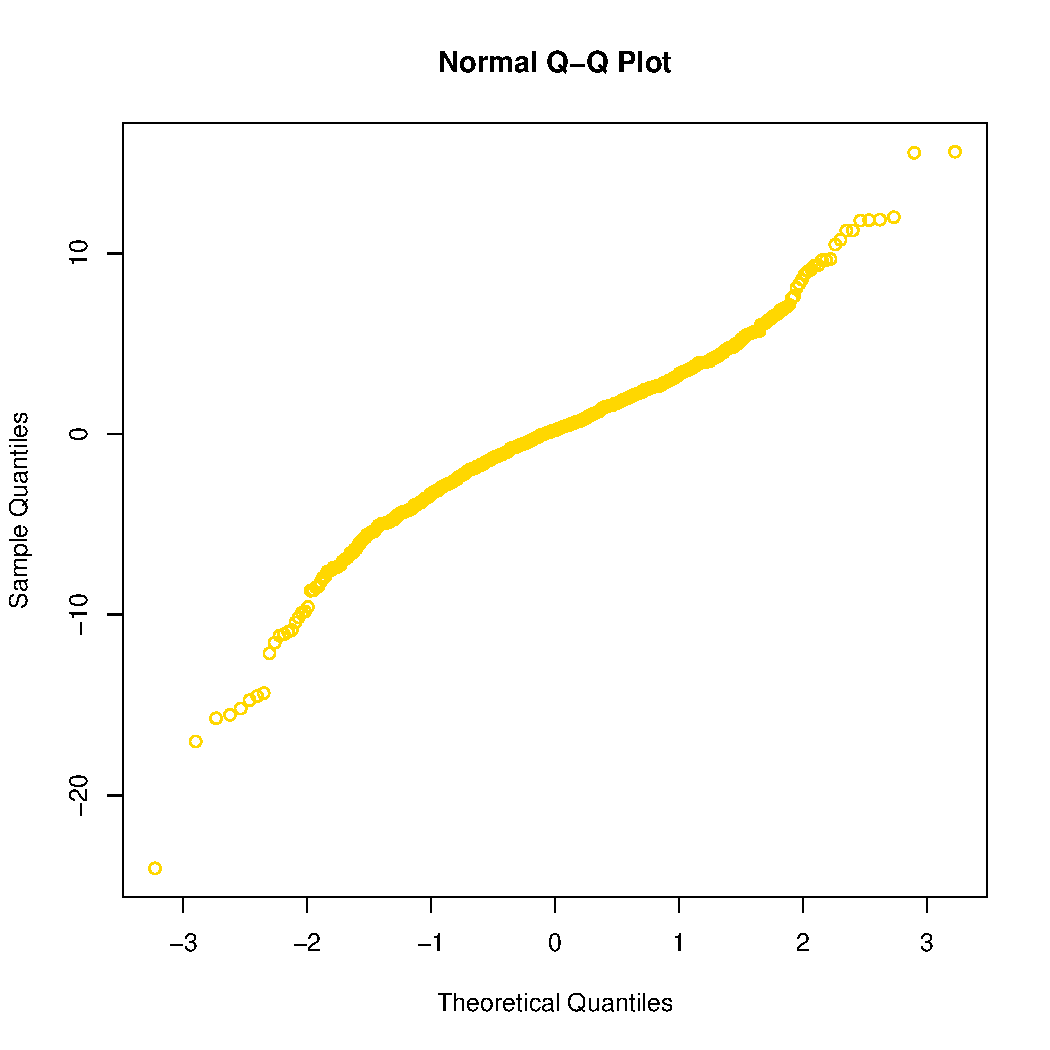
\includegraphics{raw/qqnorm.pdf}
    A plot of the histogram of the residuals shows that the residuals are normally
    distributed with mean 0 and covariance matrix $V = \sigma^2\bm R + \tau^2\bm I$
    (see Figure 3).
    \begin{figure}\begin{center}
      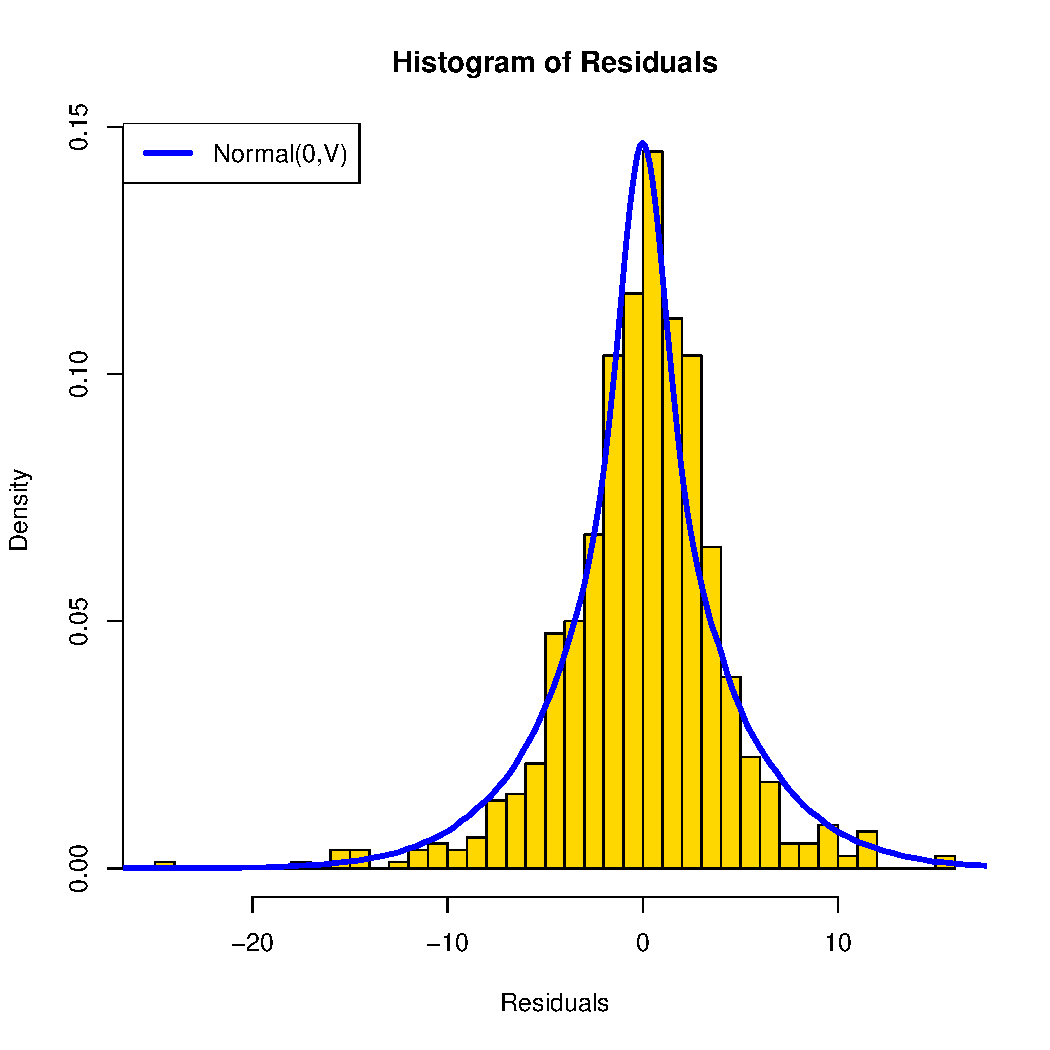
\includegraphics{raw/hist.pdf}
      \caption{Plot of histogram of residuals.}
    \end{center}\end{figure}

\section{Results}
  \subsection{Estimates of Parameters and CI}
    Estimates of the parameters are listed as follows: 
    $ \hat{\tau^2} = 19.61, \hat{\sigma^2} = 1.04, \hat{\phi} = 40.88 $.
    \textbf{Table 1} shows the parameter estimates with their 
    95\% confidence intervals.

    % latex table generated in R 3.0.2 by xtable 1.7-1 package
% Tue Mar  4 16:51:56 2014
\begin{table}[ht]
\centering
\begin{tabular}{rrrr}
  \hline
 & Estimates & CI.Lo & CI.Hi \\ 
  \hline
beta0 & 7.93766 & 1.29157 & 14.58375 \\ 
  beta1 & -0.11039 & -0.26032 & 0.03954 \\ 
  beta2 & 0.20544 & 0.06538 & 0.34549 \\ 
  beta3 & 0.08400 & -0.04960 & 0.21761 \\ 
  beta4 & 0.20130 & 0.06727 & 0.33534 \\ 
  beta5 & -0.11577 & -0.24077 & 0.00924 \\ 
  beta6 & 0.17512 & 0.05527 & 0.29497 \\ 
  beta7 & 0.14480 & 0.01922 & 0.27037 \\ 
  beta8 & 0.09521 & -0.01989 & 0.21031 \\ 
  beta9 & 0.06374 & -0.06132 & 0.18880 \\ 
  beta10 & 0.04647 & -0.06892 & 0.16187 \\ 
   \hline
\end{tabular}
\end{table}

    
    $\beta_0$ is the expected O$_3$ level if the 10 nearest CMAQ measurements are
    0. 

  \subsection{Coverage \& MSE }
    % latex table generated in R 3.0.2 by xtable 1.7-1 package
% Tue Mar  4 16:35:59 2014
\begin{table}[ht]
\centering
\begin{tabular}{rrrr}
  \hline
 & Estimate & CI.Lower & CI.Upper \\ 
  \hline
Coverage & 0.931 & 0.913 & 0.949 \\ 
  MSE & 20979.047 & 11019.079 & 30939.014 \\ 
   \hline
\end{tabular}
\end{table}

  \subsection{Predictions \& Uncertainties}
    \begin{figure}\begin{center}
    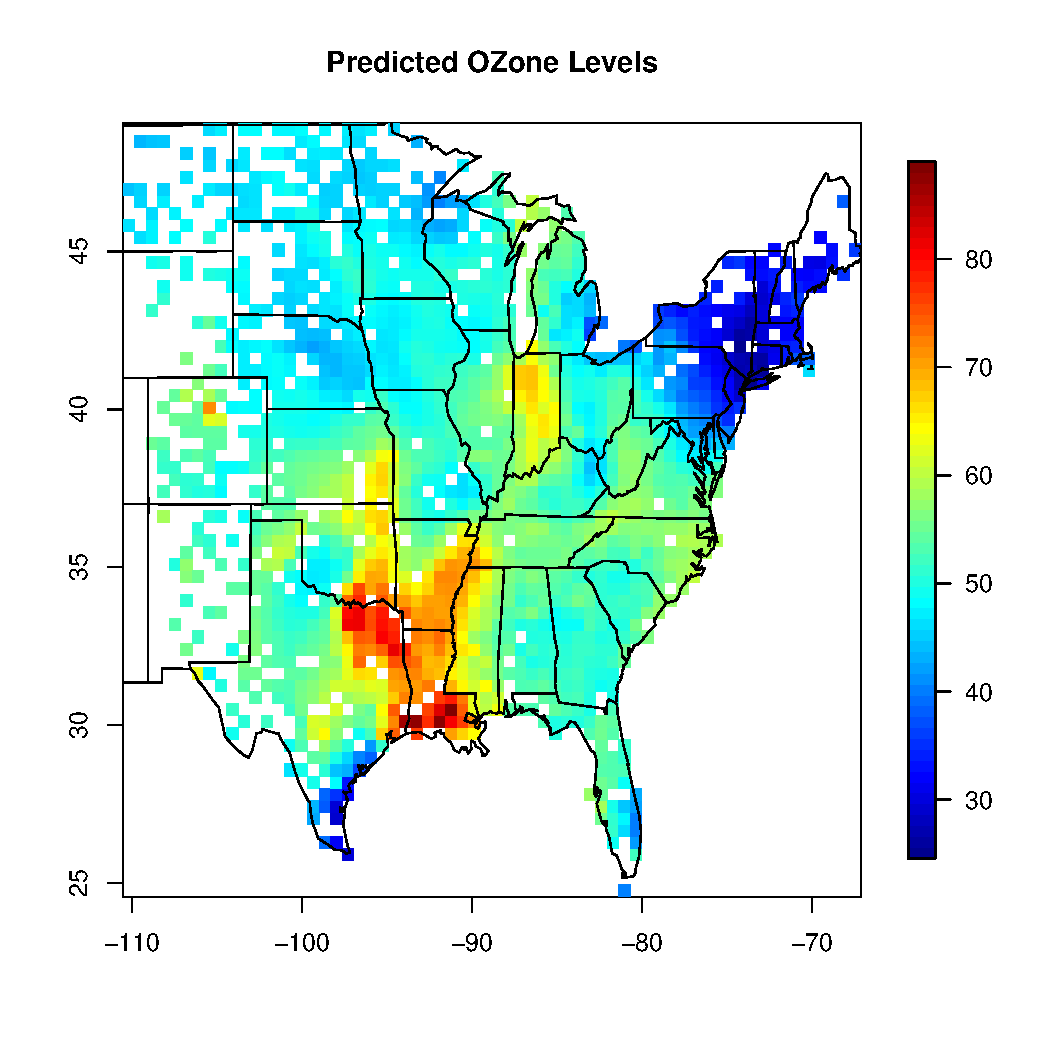
\includegraphics{raw/center.pdf}
      \caption{Predicted O$_3$.}
    \end{center}\end{figure}

    \begin{figure}\begin{center}
    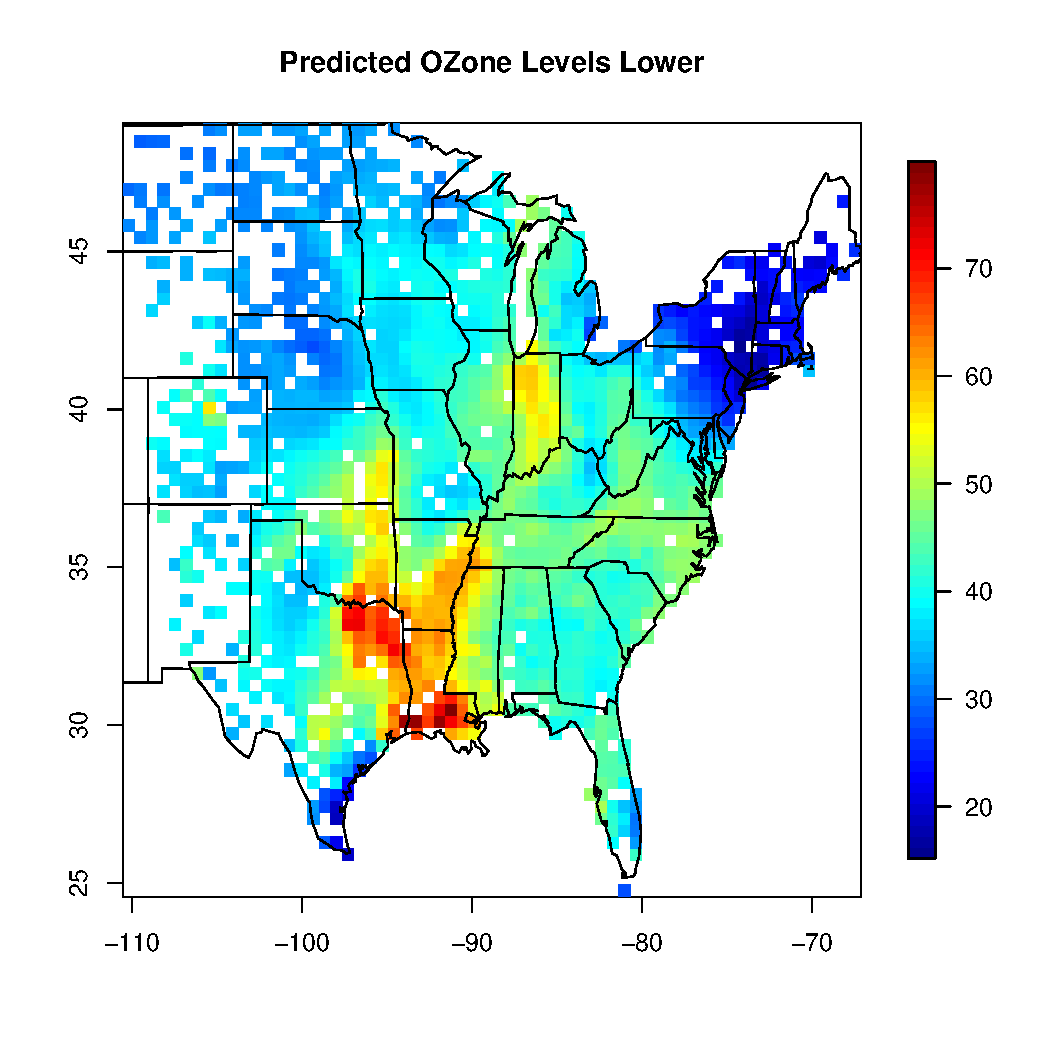
\includegraphics{raw/lower.pdf}
      \caption{Lower Predicted O$_3$.}
    \end{center}\end{figure}

    \begin{figure}\begin{center}
    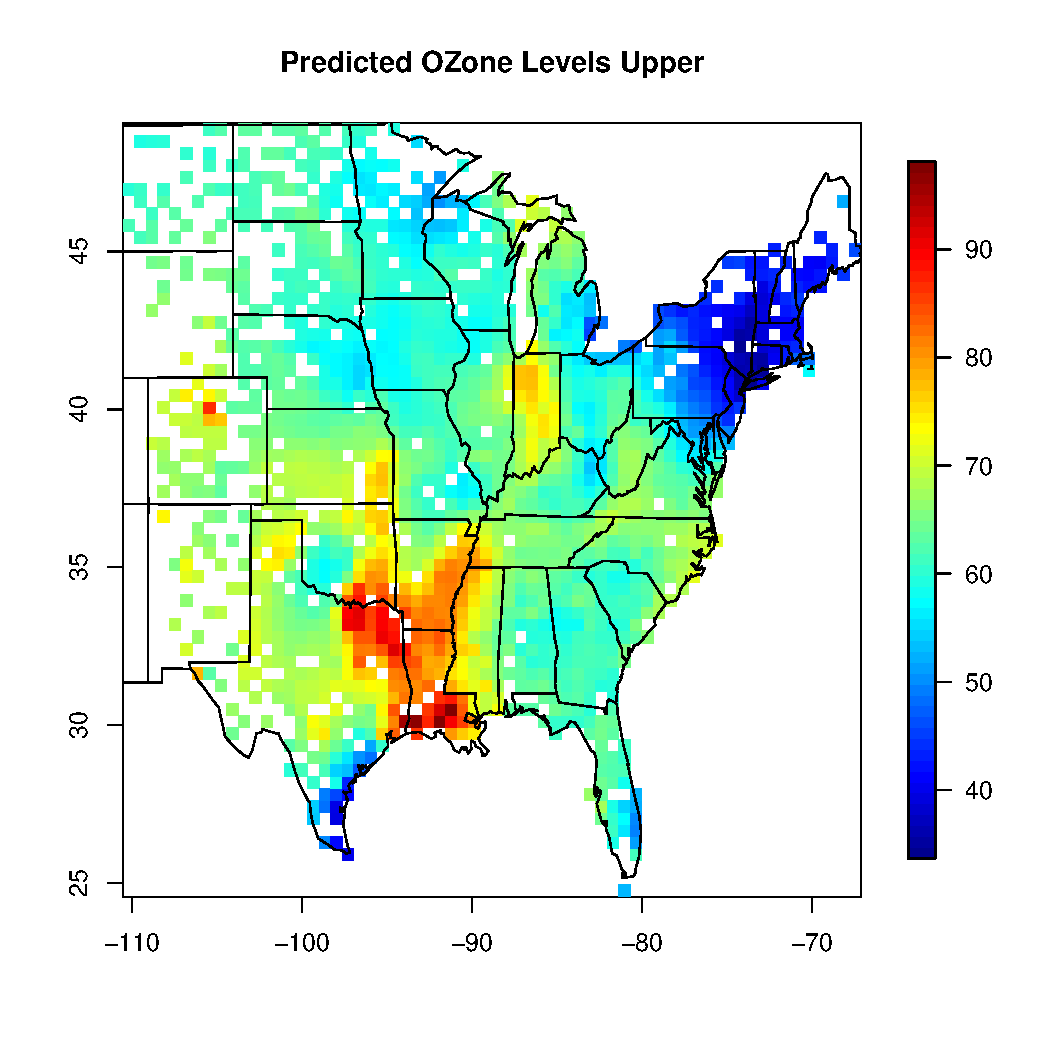
\includegraphics{raw/upper.pdf}
      \caption{Upper Predicted O$_3$.}
    \end{center}\end{figure}


  \subsection{Interpretation}
  \subsection{Summary of Main Points}
    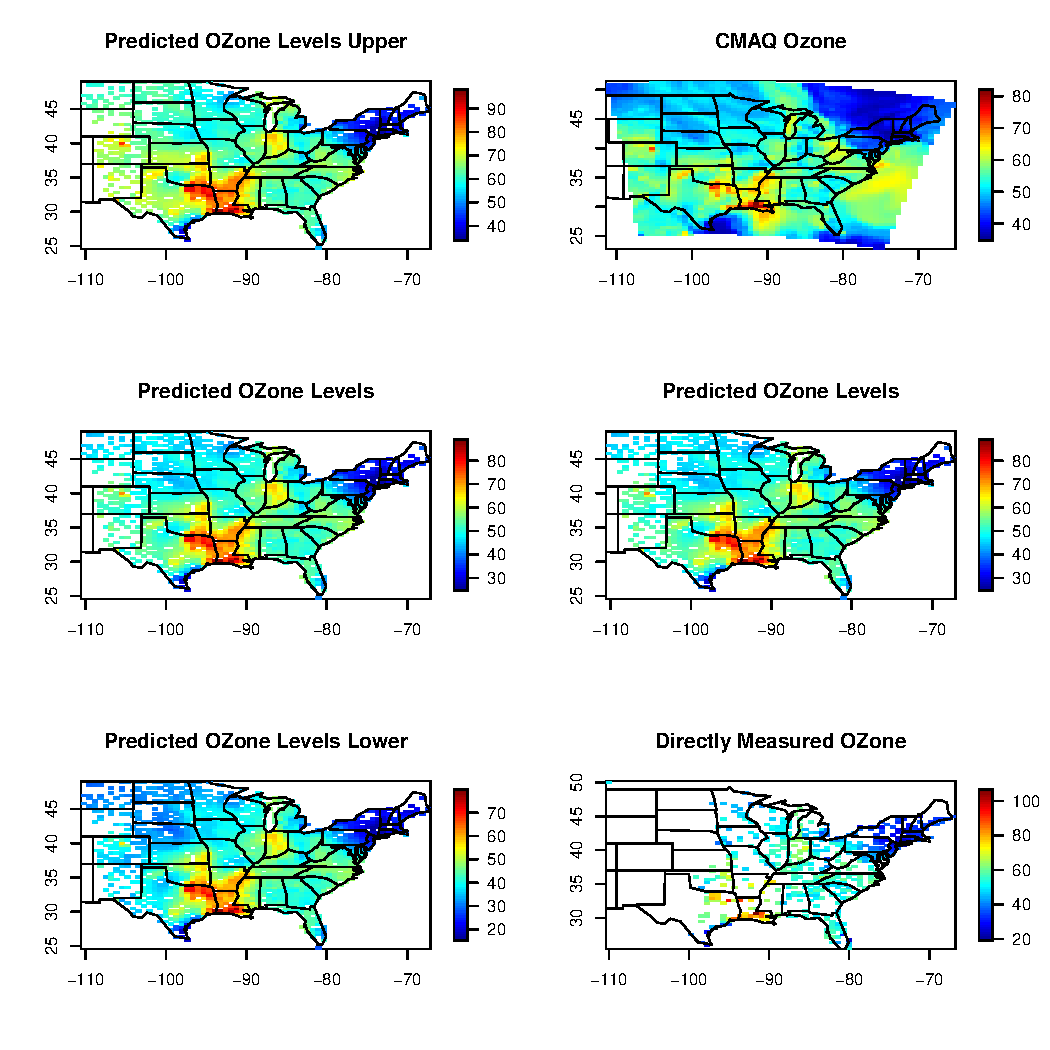
\includegraphics{raw/all.pdf}
\section{Conclusion}
  \subsection{Potential Alternative Approaches}
  \subsection{Shortcomings of GP or the way covars were chosen}
  \subsection{Further Investigation}
\end{document}
